% Year in Industry, Quarterly Report 1 (Learning Outcome 1).
% Written for a NON-TECHNICAL assessor: plain English, no jargon.
% Built on Ian's "report" LaTeX template (annotation.sty + latex-screenshot.sty).
% Build:  ./build.sh   (measures the word count with texcount, then latexmk)
% Word limit 500-750. Counted: main text, headings, table text and table captions.
% Not counted (%TC:ignore): title block, Figure 1 and its caption, references.
\documentclass[a4paper,11pt]{article}
\PassOptionsToPackage{style=authoryear, maxcitenames=1, mincitenames=1, maxbibnames=8, uniquelist=false, uniquename=false, dashed=false, useprefix=true, backend=biber}{biblatex}
\usepackage{annotation}
\usepackage{latex-screenshot}
\addbibresource{refs.bib}
\AtBeginDocument{\renewcommand*{\nameyeardelim}{\addcomma\space}}
\usetikzlibrary{arrows.meta, positioning, calc}
\usepackage{upgreek}
\usepackage{booktabs}
\usepackage{caption}
\captionsetup{font=small, labelfont=bf, margin=0.3cm}
\hfuzz=80pt
\hbadness=100000000
\setlength{\parskip}{0.35em}
\setlength{\headheight}{14pt}
\lhead{\small Year in Industry \textperiodcentered{} Quarterly Report 1}
\input{wordcount}
%TC:macro \parencite [ignore]
%TC:macro \textcite [ignore]
%TC:envir table [] text
%TC:envir tabularx [ignore,ignore] text
\hypersetup{pdftitle={Year in Industry Quarterly Report 1: Applying and developing engineering knowledge}, pdfauthor={Ian Poon}}
\newcommand{\lbl}[1]{\textbf{#1}\ }

%TC:ignore
\title{Year in Industry Quarterly Report 1:\\[2pt] \Large Applying and developing engineering knowledge}
\author[1]{Ian Poon}
\affil[1]{MEng Biomedical Engineering, Department of Bioengineering, Imperial College London}
\date{November 2026}
%TC:endignore

\begin{document}
%TC:ignore
\begin{center}
{\LARGE Year in Industry Quarterly Report 1\par}\vspace{3pt}
{\Large Applying and developing engineering knowledge\par}\vspace{8pt}
{\large Ian Poon \textperiodcentered{} November 2026\par}\vspace{2pt}
{\normalsize MEng Biomedical Engineering, Department of Bioengineering, Imperial College London\par}
\vspace{6pt}
\small
\begin{tabularx}{0.94\textwidth}{@{}lL@{}}
\toprule
Placement & Hekstra Lab, Harvard University, Cambridge MA (USA) \\
Supervisors & Doeke Hekstra (head of the lab) and Micheal Schnebly (day-to-day mentor) \\
Period covered & Quarter 1: July to October 2026 \\
Learning outcome & 1. Apply and develop engineering knowledge to the analysis, design and solution of problems \\
Word count & \wordcount{} (main text, headings, tables, table captions and in-text citations; excludes this title block, Figure~1 and references) \\
\bottomrule
\end{tabularx}
\end{center}
%TC:endignore

\section*{Context}
Proteins are the tiny machines of our cells, and force changes their shape, which is partly how we sense touch. My placement lab clips DNA onto two chemical ``hooks'' on a protein; a second strand stiffens it into a spring pushing like a drawn bow \parencite{boral2026}. The goal is a ring: DNA joined at both ends to one protein. I worked on a glowing jellyfish protein and PP2A, an enzyme that switches other proteins off, and set up 3D image analysis.

\section*{1. Using knowledge from my degree}
\begin{table}[H]
\centering\small
\caption{How I used my Year 3 modules.}\label{tab:modules}
\begin{tabularx}{\textwidth}{@{}>{\raggedright\arraybackslash}p{0.3\textwidth}L@{}}
\toprule
Module & How I used it \\
\midrule
Cellular and Molecular Mechanotransduction (how cells sense force) & Force-measuring tools cannot see shape, the gap our springs fill; proteins reshape at forces as tiny as my springs' \parencite{delrio2009}. \\
Biomedical Instrumentation; Image Processing & Microscope blur behaves like the electronic filters I analysed; 3D models are rebuilt like hospital CT scans. \\
Digital Biosignal Processing; Probability, Statistics and Data Analysis & Averaging repeated runs beats noise; I dismissed a simulated change within normal variation. \\
Modelling in Biology; Bioengineering Group Project & Computer-cluster experience for my simulations; seeing that DNA can bend smoothly or kink. \\
\bottomrule
\end{tabularx}
\end{table}

Wider reading filled gaps. Sixteen times more glowing protein gave only eleven times more glow: concentrated samples soak up light like tinted glass \parencite{lakowicz2006}, so I designed a measure unaffected by amount. My simulations gave five times a textbook model's force \parencite{zocchi2018} because the model assumes DNA kinks like a bent straw; mine bent smoothly.

\lbl{Reflection.}The modules (Table~\ref{tab:modules}) gave frameworks, not recipes, and mattered most where data broke a tidy assumption. But I have used statistics mainly to judge results, not yet to plan experiments (action A1).

\section*{2. Developing new skills and knowledge}
Beyond my Foundations of Synthetic Biology practicals, I had almost no lab experience. I learned to purify proteins and built atom-by-atom computer simulations from scratch. From recent papers I taught myself cryo-electron microscopy analysis, which turns thousands of faint images of frozen proteins into a 3D model, and set it up for the lab. I tested myself by re-analysing a 2025 study's data, matching its results almost exactly \parencite{day2025}, then taught the lab.

\lbl{Reflection.}Re-analysing, then teaching, exposed gaps that reading hid: following an explanation is not rebuilding it. But that was someone else's clean data; the real test is our own samples (A4).

\section*{3. Scoping, managing and delivering the project}
\lbl{Scoping.}Each protein has three work packages (make, test, simulate); I recorded where each stood and set my deliverables. Nothing can be tested without the ring, so making PP2A came first.

\lbl{Cost and risk.}I trialled a new filter on a cheap stand-in before risking expensive DNA.

\lbl{Contingency.}When a microscope breakdown cancelled imaging two days before my 29~October milestone talk, I presented published data instead.

\lbl{Reflection.}My planning was reactive. My group-project report had urged checking inputs before committing resources \parencite{kumar2026}, yet a mislabelled tube forced me to estimate amounts, and unplanned liquid volumes left one product too diluted to see. A lesson written down is not yet a routine (A2, A3).

\section*{4. Problem solving and creative thinking}
The old PP2A method made only a wrong, two-protein loop; a correct ring had never been made in the lab (Figure~\ref{fig:chain}). My mentor's notebook showed the protein still carried a bulky ``handle'' left over from purification. Suspecting it blocked a hook, I cut it off; a new DNA-containing product appeared. But a ring weighs the same as DNA hanging by one end, so I used a filter that only lets rings through: beads that grab any free hook. Ours passed: the lab's first correct PP2A ring.

\lbl{Reflection.}\textit{Strength:} each step tested one clear idea, and when weighing failed I found another question to ask. \textit{Weakness:} one change at a time is slow and can hide factors that interact; one additive stops clumping but blocks attachment (A1).

%TC:ignore
\begin{figure}[t]
\centering
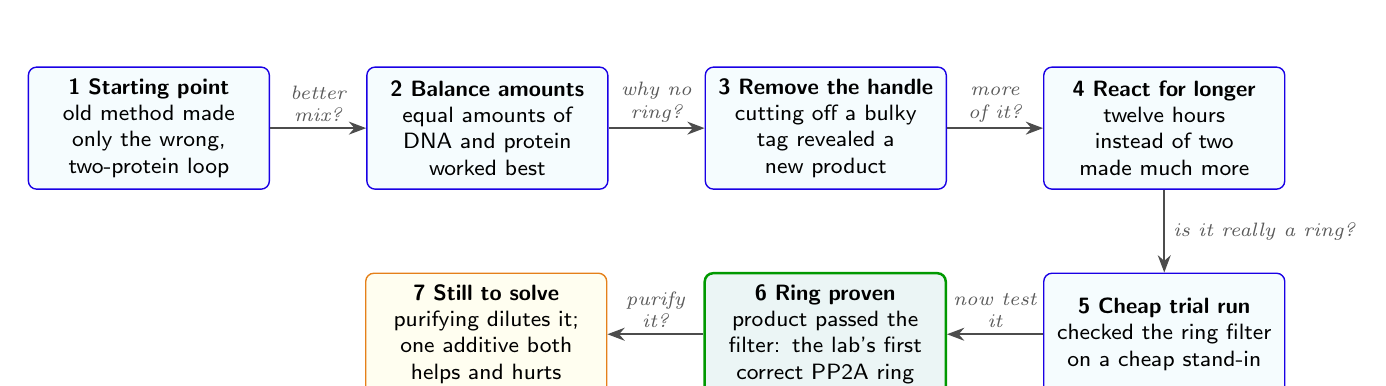
\begin{tikzpicture}[
  font=\footnotesize\sffamily, execute at begin node={\hyphenpenalty=10000},
  stage/.style={draw=blue!90!red, fill=cyan!4, line width=0.5pt, rounded corners=3pt,
               text width=2.85cm, minimum height=1.55cm, align=center, inner sep=3pt},
  win/.style={stage, draw=green!60!black, fill=teal!8, line width=0.9pt},
  open/.style={stage, draw=orange!60!brown, fill=yellow!6},
  q/.style={font=\scriptsize\itshape, text=black!65, align=center, inner sep=1pt},
  arr/.style={-{Stealth[length=2.2mm]}, line width=0.6pt, draw=black!70},
  node distance=0.62cm and 1.22cm]
  \node[stage] (a) {\textbf{1 Starting point}\\ old method made only the wrong, two-protein loop};
  \node[stage, right=of a] (b) {\textbf{2 Balance amounts}\\ equal amounts of DNA and protein worked best};
  \node[stage, right=of b] (c) {\textbf{3 Remove the handle}\\ cutting off a bulky tag revealed a new product};
  \node[stage, right=of c] (d) {\textbf{4 React for longer}\\ twelve hours instead of two made much more};
  \node[stage, below=1.05cm of d] (e) {\textbf{5 Cheap trial run}\\ checked the ring filter on a cheap stand-in};
  \node[win, left=of e] (f) {\textbf{6 Ring proven}\\ product passed the filter: the lab's first correct PP2A ring};
  \node[open, left=of f] (g) {\textbf{7 Still to solve}\\ purifying dilutes it; one additive both helps and hurts};
  \draw[arr] (a) -- node[q, above=1pt]{better\\mix?} (b);
  \draw[arr] (b) -- node[q, above=1pt]{why no\\ring?} (c);
  \draw[arr] (c) -- node[q, above=1pt]{more\\of it?} (d);
  \draw[arr] (d) -- node[q, right=2pt]{is it really a ring?} (e);
  \draw[arr] (e) -- node[q, above=1pt]{now test\\it} (f);
  \draw[arr] (f) -- node[q, above=1pt]{purify\\it?} (g);
\end{tikzpicture}
\caption{How I made the lab's first correct ring-shaped PP2A spring. Each experiment tested one idea, and its result set the next question (full technical detail in \textcite{poon2026}). Green marks the milestone; amber marks the problems still open, which actions A1 and A3 address.}
\label{fig:chain}
\end{figure}
%TC:endignore

\section*{Personal action plan}
Reflecting across all sections \parencite{moon2006} reveals a pattern: I explain surprises well but anticipate them poorly.

\begin{table}[H]
\centering\small
\caption{My action plan.}\label{tab:plan}
\begin{tabularx}{\textwidth}{@{}lLll@{}}
\toprule
& Action & From & By \\
\midrule
A1 & Tune the remaining PP2A steps together, varying several factors at once & \S1, \S4 & Dec 2026 \\
A2 & Check every ready-made solution's strength before use & \S3 & Now \\
A3 & One-page plan per work package (milestones, volumes, fallback), reviewed monthly with my mentor & \S3 & Nov 2026 \\
A4 & Publish my analysis guide; run it on our own samples & \S2 & Jan 2027 \\
\bottomrule
\end{tabularx}
\end{table}

%TC:ignore
\printbibliography
%TC:endignore
\end{document}
